% Trailing asterisk to suppress section number
\section*{Task 1: SQL injections}

\subsection*{Exercises:}
\begin{enumerate}
\item The result shows below:
	\par 
	\begin{center}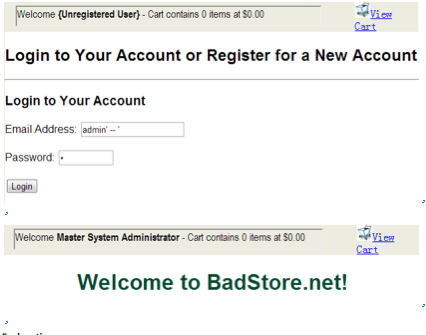
\includegraphics[height=2.5in]{sqli1}
	\end{center}
	Explanation: Before injection, the SQL code should be SELECT * FROM user WHERE EmailAddress = 'emailaddress’ AND Password = ’password’. Then during the injection, we input admin ‘--‘ in the text of Email Address and whatever password is in the text of Password. The WHERE condition is altered into WHERE EmailAddress = 'admin' -- ' AND 	Password = ’password’ (WHERE EmailAddress = 'admin'). So there is no need of password and we can directly log into admin account.
\item The result shows below (Continued on next page):
	\par
	\begin{center}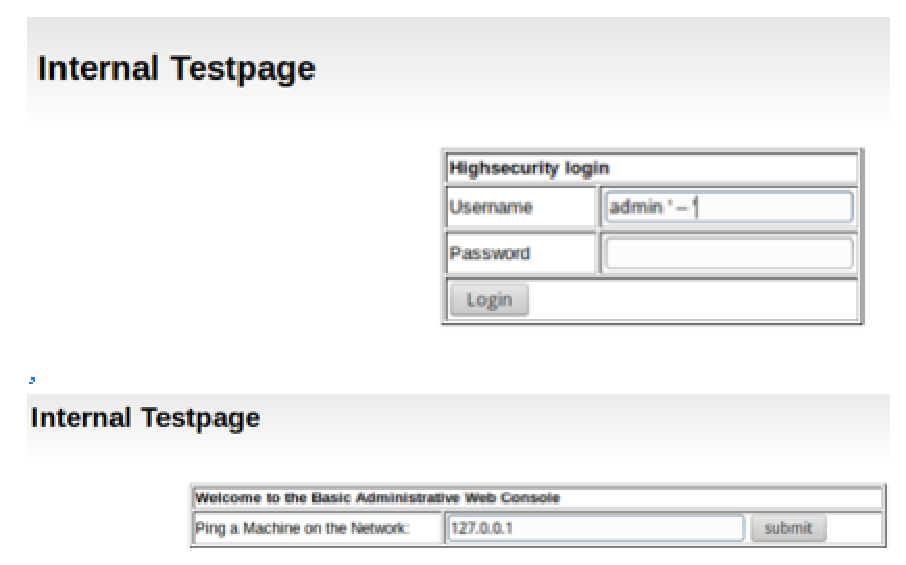
\includegraphics[height=2.5in]{sqli2}
	\end{center}
	Explanation:Before injection, the SQL code should be SELECT * FROM user WHERE UserName = 'username’ AND Password = ’password’. Then during the injection, we input admin ‘--‘ in the text of Username and whatever password is in the text of Password. The WHERE condition is altered into WHERE UserName = 'admin' -- ' AND Password = ’password’ (WHERE UserName = 'admin'). So there is no need of password and we can directly log into admin account.
\item \textbf{Prepared Statement} 
	\par Prepared statement is also called parametrized statement, which is a SQL query with variables inside of it. That is to say, we prepare the query with blank spot to fill and it will automatically protect the query from SQL injection.
	\par Here is the example:
	\par \textit{stmt = dbh->prepare(“INSERT INTO REGISTRY (name, value) VALUES (:name, :value)”);}
	\par \textit{stmt->bindParam(':name', name);}
	\par \textit{stmt->bindParam(':value', value);}
	\par In our case, we can create prepared statement as follows:
prepare(“SELECT * FROM user WHERE UserName = :username AND Password = :password”);
bind(':username', username);
bind(':password', password);
	\par
	\par \textbf{Explanation}
	\par Before injection, we have two variables, admin(username) and test(password). The SQL query should be SELECT * FROM user WHERE username = ‘admin’ AND password = ‘test’. Then during the injection, these two variables are changed into admin' --(username) and 123(password) and the SQL query becomes SELECT * FROM user WHERE username = 'admin\' --' AND password = '123'. It’s because the binding system will automatically change the input to protect the query. So the SQL injection doesn't work in this situation.
\item The school lost all the student records because the table Students in the database is dropped by SQL injection. Before injection, the SQL code should be INSERT INTO Students VALUES ('Robert'). Then during the injection, the query is altered into INSERT INTO Students VALUES ('Robert'); DROP TABLE Students; -- . So after the query is executed, the table Students will be dropped automatically.

What the school should do is to sanitize the database inputs by utilizing prepared statement as mentioned above. They can create prepared statement as follows:
prepare(“INSERT INTO Students VALUES (':name')”);
bind(':name',name);

\end{enumerate}
